\documentclass[1p]{elsarticle_modified}
%\bibliographystyle{elsarticle-num}

%\usepackage[colorlinks]{hyperref}
%\usepackage{abbrmath_seonhwa} %\Abb, \Ascr, \Acal ,\Abf, \Afrak
\usepackage{amsfonts}
\usepackage{amssymb}
\usepackage{amsmath}
\usepackage{amsthm}
\usepackage{scalefnt}
\usepackage{amsbsy}
\usepackage{kotex}
\usepackage{caption}
\usepackage{subfig}
\usepackage{color}
\usepackage{graphicx}
\usepackage{xcolor} %% white, black, red, green, blue, cyan, magenta, yellow
\usepackage{float}
\usepackage{setspace}
\usepackage{hyperref}

\usepackage{tikz}
\usetikzlibrary{arrows}

\usepackage{multirow}
\usepackage{array} % fixed length table
\usepackage{hhline}

%%%%%%%%%%%%%%%%%%%%%
\makeatletter
\renewcommand*\env@matrix[1][\arraystretch]{%
	\edef\arraystretch{#1}%
	\hskip -\arraycolsep
	\let\@ifnextchar\new@ifnextchar
	\array{*\c@MaxMatrixCols c}}
\makeatother %https://tex.stackexchange.com/questions/14071/how-can-i-increase-the-line-spacing-in-a-matrix
%%%%%%%%%%%%%%%

\usepackage[normalem]{ulem}

\newcommand{\msout}[1]{\ifmmode\text{\sout{\ensuremath{#1}}}\else\sout{#1}\fi}
%SOURCE: \msout is \stkout macro in https://tex.stackexchange.com/questions/20609/strikeout-in-math-mode

\newcommand{\cancel}[1]{
	\ifmmode
	{\color{red}\msout{#1}}
	\else
	{\color{red}\sout{#1}}
	\fi
}

\newcommand{\add}[1]{
	{\color{blue}\uwave{#1}}
}

\newcommand{\replace}[2]{
	\ifmmode
	{\color{red}\msout{#1}}{\color{blue}\uwave{#2}}
	\else
	{\color{red}\sout{#1}}{\color{blue}\uwave{#2}}
	\fi
}

\newcommand{\Sol}{\mathcal{S}} %segment
\newcommand{\D}{D} %diagram
\newcommand{\A}{\mathcal{A}} %arc


%%%%%%%%%%%%%%%%%%%%%%%%%%%%%5 test

\def\sl{\operatorname{\textup{SL}}(2,\Cbb)}
\def\psl{\operatorname{\textup{PSL}}(2,\Cbb)}
\def\quan{\mkern 1mu \triangleright \mkern 1mu}

\theoremstyle{definition}
\newtheorem{thm}{Theorem}[section]
\newtheorem{prop}[thm]{Proposition}
\newtheorem{lem}[thm]{Lemma}
\newtheorem{ques}[thm]{Question}
\newtheorem{cor}[thm]{Corollary}
\newtheorem{defn}[thm]{Definition}
\newtheorem{exam}[thm]{Example}
\newtheorem{rmk}[thm]{Remark}
\newtheorem{alg}[thm]{Algorithm}

\newcommand{\I}{\sqrt{-1}}
\begin{document}

%\begin{frontmatter}
%
%\title{Boundary parabolic representations of knots up to 8 crossings}
%
%%% Group authors per affiliation:
%\author{Yunhi Cho} 
%\address{Department of Mathematics, University of Seoul, Seoul, Korea}
%\ead{yhcho@uos.ac.kr}
%
%
%\author{Seonhwa Kim} %\fnref{s_kim}}
%\address{Center for Geometry and Physics, Institute for Basic Science, Pohang, 37673, Korea}
%\ead{ryeona17@ibs.re.kr}
%
%\author{Hyuk Kim}
%\address{Department of Mathematical Sciences, Seoul National University, Seoul 08826, Korea}
%\ead{hyukkim@snu.ac.kr}
%
%\author{Seokbeom Yoon}
%\address{Department of Mathematical Sciences, Seoul National University, Seoul, 08826,  Korea}
%\ead{sbyoon15@snu.ac.kr}
%
%\begin{abstract}
%We find all boundary parabolic representation of knots up to 8 crossings.
%
%\end{abstract}
%\begin{keyword}
%    \MSC[2010] 57M25 
%\end{keyword}
%
%\end{frontmatter}

%\linenumbers
%\tableofcontents
%
\newcommand\colored[1]{\textcolor{white}{\rule[-0.35ex]{0.8em}{1.4ex}}\kern-0.8em\color{red} #1}%
%\newcommand\colored[1]{\textcolor{white}{ #1}\kern-2.17ex	\textcolor{white}{ #1}\kern-1.81ex	\textcolor{white}{ #1}\kern-2.15ex\color{red}#1	}

{\Large $\underline{12n_{0497}~(K12n_{0497})}$}

\setlength{\tabcolsep}{10pt}
\renewcommand{\arraystretch}{1.6}
\vspace{1cm}\begin{tabular}{m{100pt}>{\centering\arraybackslash}m{274pt}}
\multirow{5}{120pt}{
	\centering
	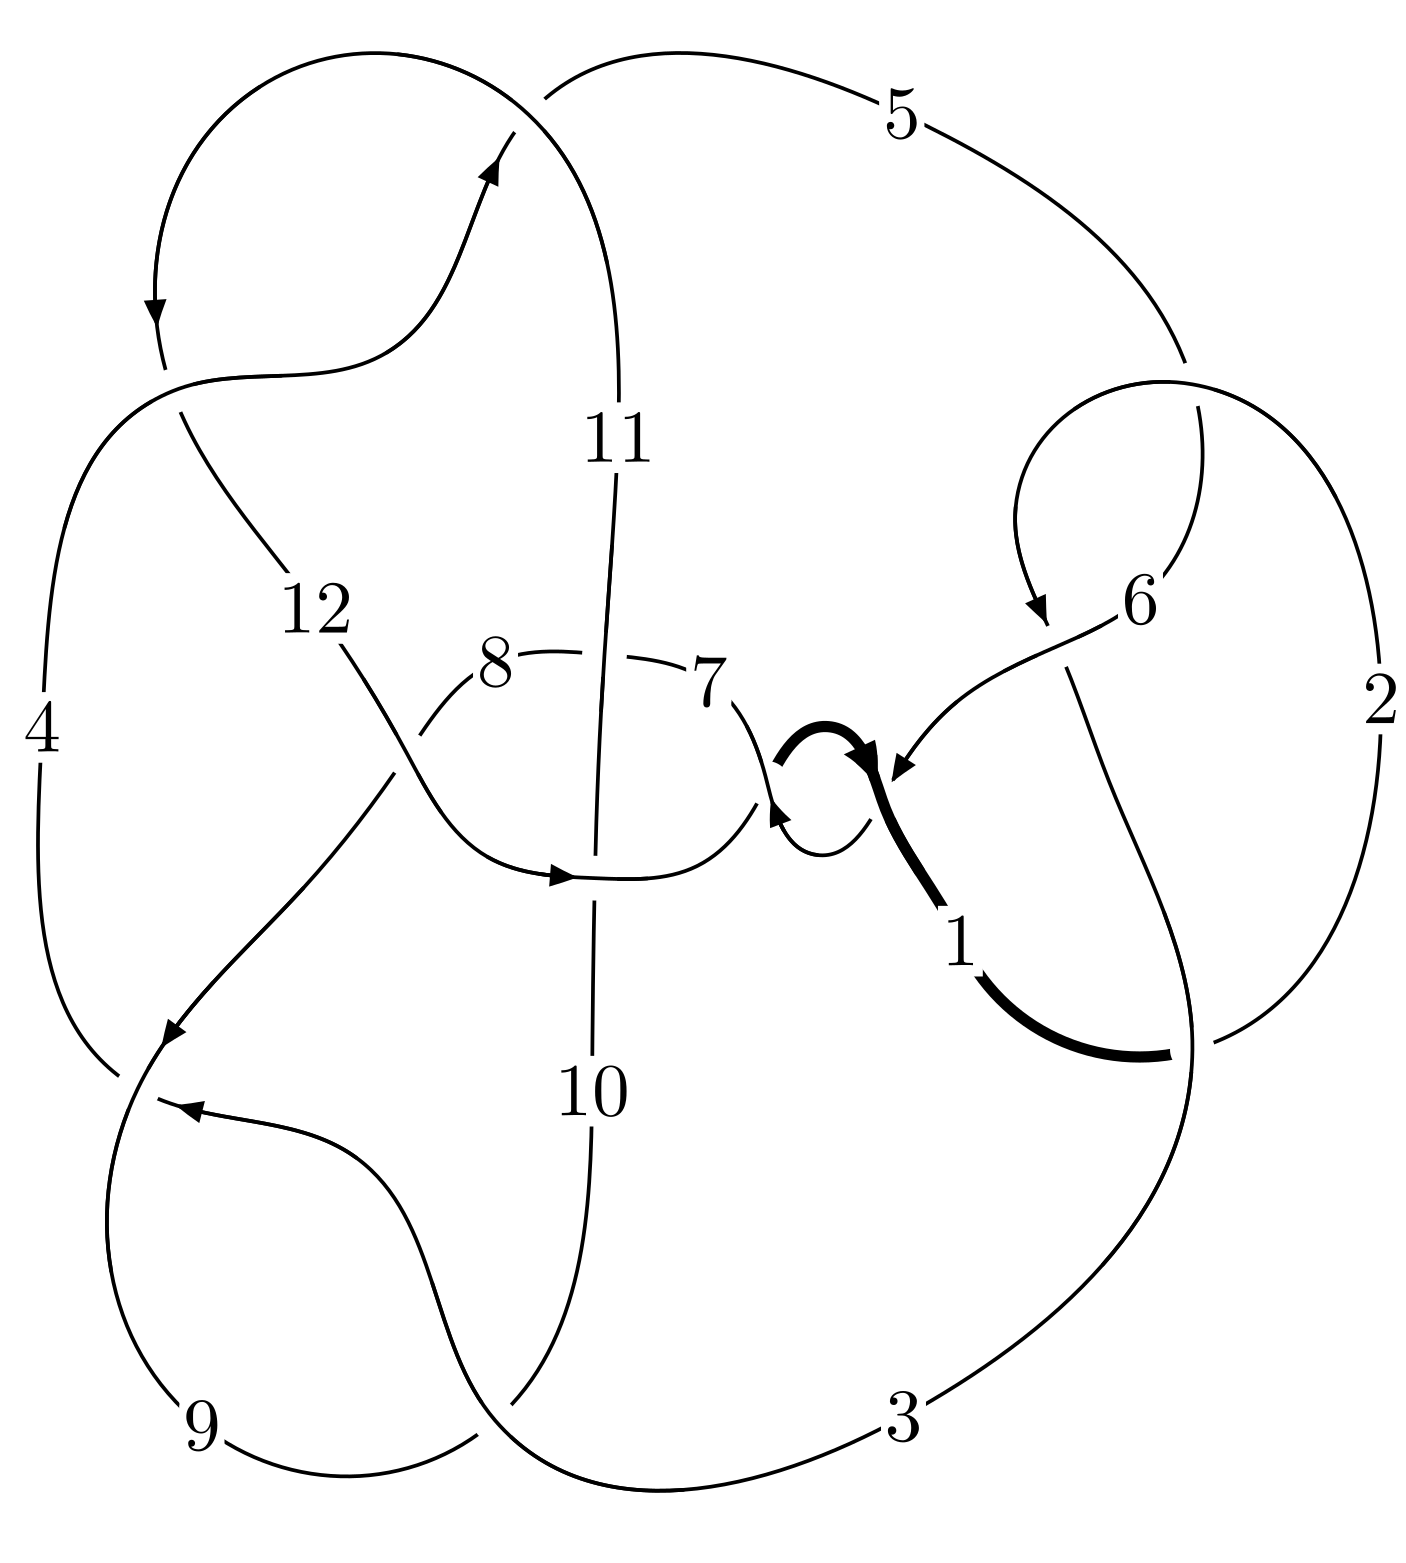
\includegraphics[width=112pt]{../../../GIT/diagram.site/Diagrams/png/2586_12n_0497.png}\\
\ \ \ A knot diagram\footnotemark}&
\allowdisplaybreaks
\textbf{Linearized knot diagam} \\
\cline{2-2}
 &
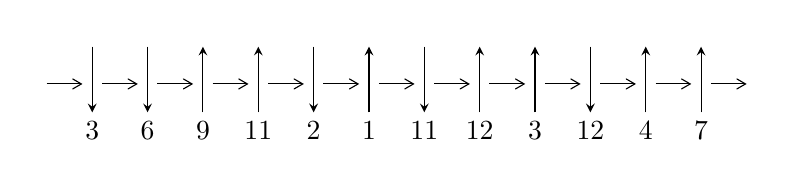
\begin{tikzpicture}[x=20pt, y=17pt]
	% nodes
	\node (C0) at (0, 0) {};
	\node (C1) at (1, 0) {};
	\node (C1U) at (1, +1) {};
	\node (C1D) at (1, -1) {3};

	\node (C2) at (2, 0) {};
	\node (C2U) at (2, +1) {};
	\node (C2D) at (2, -1) {6};

	\node (C3) at (3, 0) {};
	\node (C3U) at (3, +1) {};
	\node (C3D) at (3, -1) {9};

	\node (C4) at (4, 0) {};
	\node (C4U) at (4, +1) {};
	\node (C4D) at (4, -1) {11};

	\node (C5) at (5, 0) {};
	\node (C5U) at (5, +1) {};
	\node (C5D) at (5, -1) {2};

	\node (C6) at (6, 0) {};
	\node (C6U) at (6, +1) {};
	\node (C6D) at (6, -1) {1};

	\node (C7) at (7, 0) {};
	\node (C7U) at (7, +1) {};
	\node (C7D) at (7, -1) {11};

	\node (C8) at (8, 0) {};
	\node (C8U) at (8, +1) {};
	\node (C8D) at (8, -1) {12};

	\node (C9) at (9, 0) {};
	\node (C9U) at (9, +1) {};
	\node (C9D) at (9, -1) {3};

	\node (C10) at (10, 0) {};
	\node (C10U) at (10, +1) {};
	\node (C10D) at (10, -1) {12};

	\node (C11) at (11, 0) {};
	\node (C11U) at (11, +1) {};
	\node (C11D) at (11, -1) {4};

	\node (C12) at (12, 0) {};
	\node (C12U) at (12, +1) {};
	\node (C12D) at (12, -1) {7};
	\node (C13) at (13, 0) {};

	% arrows
	\draw[->,>={angle 60}]
	(C0) edge (C1) (C1) edge (C2) (C2) edge (C3) (C3) edge (C4) (C4) edge (C5) (C5) edge (C6) (C6) edge (C7) (C7) edge (C8) (C8) edge (C9) (C9) edge (C10) (C10) edge (C11) (C11) edge (C12) (C12) edge (C13) ;	\draw[->,>=stealth]
	(C1U) edge (C1D) (C2U) edge (C2D) (C3D) edge (C3U) (C4D) edge (C4U) (C5U) edge (C5D) (C6D) edge (C6U) (C7U) edge (C7D) (C8D) edge (C8U) (C9D) edge (C9U) (C10U) edge (C10D) (C11D) edge (C11U) (C12D) edge (C12U) ;
	\end{tikzpicture} \\
\hhline{~~} \\& 
\textbf{Solving Sequence} \\ \cline{2-2} 
 &
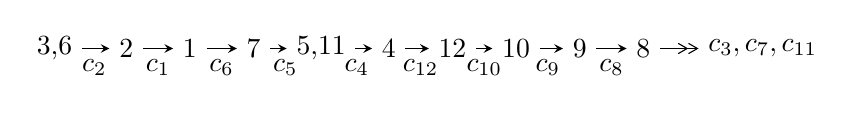
\begin{tikzpicture}[x=23pt, y=7pt]
	% node
	\node (A0) at (-1/8, 0) {3,6};
	\node (A1) at (1, 0) {2};
	\node (A2) at (2, 0) {1};
	\node (A3) at (3, 0) {7};
	\node (A4) at (65/16, 0) {5,11};
	\node (A5) at (41/8, 0) {4};
	\node (A6) at (49/8, 0) {12};
	\node (A7) at (57/8, 0) {10};
	\node (A8) at (65/8, 0) {9};
	\node (A9) at (73/8, 0) {8};
	\node (C1) at (1/2, -1) {$c_{2}$};
	\node (C2) at (3/2, -1) {$c_{1}$};
	\node (C3) at (5/2, -1) {$c_{6}$};
	\node (C4) at (7/2, -1) {$c_{5}$};
	\node (C5) at (37/8, -1) {$c_{4}$};
	\node (C6) at (45/8, -1) {$c_{12}$};
	\node (C7) at (53/8, -1) {$c_{10}$};
	\node (C8) at (61/8, -1) {$c_{9}$};
	\node (C9) at (69/8, -1) {$c_{8}$};
	\node (A10) at (11, 0) {$c_{3},c_{7},c_{11}$};

	% edge
	\draw[->,>=stealth]	
	(A0) edge (A1) (A1) edge (A2) (A2) edge (A3) (A3) edge (A4) (A4) edge (A5) (A5) edge (A6) (A6) edge (A7) (A7) edge (A8) (A8) edge (A9) ;
	\draw[->>,>={angle 60}]	
	(A9) edge (A10);
\end{tikzpicture} \\ 

\end{tabular} \\

\footnotetext{
The image of knot diagram is generated by the software ``\textbf{Draw programme}" developed by Andrew Bartholomew(\url{http://www.layer8.co.uk/maths/draw/index.htm\#Running-draw}), where we modified some parts for our purpose(\url{https://github.com/CATsTAILs/LinksPainter}).
}\phantom \\ \newline 
\centering \textbf{Ideals for irreducible components\footnotemark of $X_{\text{par}}$} 
 
\begin{align*}
I^u_{1}&=\langle 
- u^{26}+u^{25}+\cdots+b-1,\;- u^{27}+u^{26}+\cdots+2 a-1,\;u^{28}-3 u^{27}+\cdots-5 u+2\rangle \\
I^u_{2}&=\langle 
15 u^{16} a+46 u^{16}+\cdots+16 a+57,\;2 u^{16} a+2 u^{16}+\cdots+2 a+2,\\
\phantom{I^u_{2}}&\phantom{= \langle  }u^{17}+u^{16}-4 u^{15}-5 u^{14}+7 u^{13}+11 u^{12}-4 u^{11}-12 u^{10}-3 u^9+5 u^8+6 u^7+2 u^6-2 u^5-2 u^4+u+1\rangle \\
I^u_{3}&=\langle 
- u^9+u^8+2 u^7-2 u^6- u^5+2 u^4-2 u^3+b+u,\;- u^9+3 u^7-3 u^5- u^3- u^2+a+2 u+1,\\
\phantom{I^u_{3}}&\phantom{= \langle  }u^{10}-3 u^8+4 u^6- u^4- u^2+1\rangle \\
\\
\end{align*}
\raggedright * 3 irreducible components of $\dim_{\mathbb{C}}=0$, with total 72 representations.\\
\footnotetext{All coefficients of polynomials are rational numbers. But the coefficients are sometimes approximated in decimal forms when there is not enough margin.}
\newpage
\renewcommand{\arraystretch}{1}
\centering \section*{I. $I^u_{1}= \langle - u^{26}+u^{25}+\cdots+b-1,\;- u^{27}+u^{26}+\cdots+2 a-1,\;u^{28}-3 u^{27}+\cdots-5 u+2 \rangle$}
\flushleft \textbf{(i) Arc colorings}\\
\begin{tabular}{m{7pt} m{180pt} m{7pt} m{180pt} }
\flushright $a_{3}=$&$\begin{pmatrix}1\\0\end{pmatrix}$ \\
\flushright $a_{6}=$&$\begin{pmatrix}0\\u\end{pmatrix}$ \\
\flushright $a_{2}=$&$\begin{pmatrix}1\\- u^2\end{pmatrix}$ \\
\flushright $a_{1}=$&$\begin{pmatrix}- u^2+1\\- u^2\end{pmatrix}$ \\
\flushright $a_{7}=$&$\begin{pmatrix}u^5-2 u^3+u\\u^5- u^3+u\end{pmatrix}$ \\
\flushright $a_{5}=$&$\begin{pmatrix}u\\- u^3+u\end{pmatrix}$ \\
\flushright $a_{11}=$&$\begin{pmatrix}\frac{1}{2} u^{27}-\frac{1}{2} u^{26}+\cdots+\frac{1}{2} u+\frac{1}{2}\\u^{26}- u^{25}+\cdots-2 u+1\end{pmatrix}$ \\
\flushright $a_{4}=$&$\begin{pmatrix}\frac{5}{2} u^{27}-\frac{11}{2} u^{26}+\cdots+\frac{19}{2} u-\frac{7}{2}\\u^{27}-2 u^{26}+\cdots+4 u-1\end{pmatrix}$ \\
\flushright $a_{12}=$&$\begin{pmatrix}- u^8+3 u^6-3 u^4+1\\- u^8+2 u^6-2 u^4\end{pmatrix}$ \\
\flushright $a_{10}=$&$\begin{pmatrix}-\frac{1}{2} u^{27}-\frac{1}{2} u^{26}+\cdots-\frac{1}{2} u-\frac{1}{2}\\- u^{26}+u^{25}+\cdots+u-1\end{pmatrix}$ \\
\flushright $a_{9}=$&$\begin{pmatrix}-\frac{1}{2} u^{27}+\frac{1}{2} u^{26}+\cdots-\frac{3}{2} u+\frac{1}{2}\\- u^{26}+u^{25}+\cdots+u-1\end{pmatrix}$ \\
\flushright $a_{8}=$&$\begin{pmatrix}-\frac{1}{2} u^{27}+\frac{1}{2} u^{26}+\cdots-\frac{3}{2} u-\frac{1}{2}\\u^{27}-3 u^{26}+\cdots+4 u-3\end{pmatrix}$\\&\end{tabular}
\flushleft \textbf{(ii) Obstruction class $= -1$}\\~\\
\flushleft \textbf{(iii) Cusp Shapes $= 12 u^{27}-26 u^{26}-60 u^{25}+194 u^{24}+66 u^{23}-624 u^{22}+300 u^{21}+1000 u^{20}-1212 u^{19}-496 u^{18}+1882 u^{17}-990 u^{16}-1108 u^{15}+1922 u^{14}-632 u^{13}-1070 u^{12}+1352 u^{11}-364 u^{10}-552 u^9+642 u^8-188 u^7-148 u^6+140 u^5-26 u^4-4 u^3-26 u^2+40 u-18$}\\~\\
\newpage\renewcommand{\arraystretch}{1}
\flushleft \textbf{(iv) u-Polynomials at the component}\newline \\
\begin{tabular}{m{50pt}|m{274pt}}
Crossings & \hspace{64pt}u-Polynomials at each crossing \\
\hline $$\begin{aligned}c_{1}\end{aligned}$$&$\begin{aligned}
&u^{28}+15 u^{27}+\cdots+5 u+4
\end{aligned}$\\
\hline $$\begin{aligned}c_{2},c_{5}\end{aligned}$$&$\begin{aligned}
&u^{28}+3 u^{27}+\cdots+5 u+2
\end{aligned}$\\
\hline $$\begin{aligned}c_{3},c_{4},c_{9}\\c_{11}\end{aligned}$$&$\begin{aligned}
&u^{28}+4 u^{26}+\cdots+4 u^2+1
\end{aligned}$\\
\hline $$\begin{aligned}c_{6},c_{12}\end{aligned}$$&$\begin{aligned}
&u^{28}+9 u^{27}+\cdots+131 u+22
\end{aligned}$\\
\hline $$\begin{aligned}c_{7},c_{10}\end{aligned}$$&$\begin{aligned}
&u^{28}+8 u^{27}+\cdots+8 u+1
\end{aligned}$\\
\hline $$\begin{aligned}c_{8}\end{aligned}$$&$\begin{aligned}
&u^{28}-27 u^{27}+\cdots-1310720 u+131072
\end{aligned}$\\
\hline
\end{tabular}\\~\\
\newpage\renewcommand{\arraystretch}{1}
\flushleft \textbf{(v) Riley Polynomials at the component}\newline \\
\begin{tabular}{m{50pt}|m{274pt}}
Crossings & \hspace{64pt}Riley Polynomials at each crossing \\
\hline $$\begin{aligned}c_{1}\end{aligned}$$&$\begin{aligned}
&y^{28}-3 y^{27}+\cdots+127 y+16
\end{aligned}$\\
\hline $$\begin{aligned}c_{2},c_{5}\end{aligned}$$&$\begin{aligned}
&y^{28}-15 y^{27}+\cdots-5 y+4
\end{aligned}$\\
\hline $$\begin{aligned}c_{3},c_{4},c_{9}\\c_{11}\end{aligned}$$&$\begin{aligned}
&y^{28}+8 y^{27}+\cdots+8 y+1
\end{aligned}$\\
\hline $$\begin{aligned}c_{6},c_{12}\end{aligned}$$&$\begin{aligned}
&y^{28}+21 y^{27}+\cdots+4619 y+484
\end{aligned}$\\
\hline $$\begin{aligned}c_{7},c_{10}\end{aligned}$$&$\begin{aligned}
&y^{28}+36 y^{27}+\cdots-4 y+1
\end{aligned}$\\
\hline $$\begin{aligned}c_{8}\end{aligned}$$&$\begin{aligned}
&y^{28}- y^{27}+\cdots-68719476736 y+17179869184
\end{aligned}$\\
\hline
\end{tabular}\\~\\
\newpage\flushleft \textbf{(vi) Complex Volumes and Cusp Shapes}
$$\begin{array}{c|c|c}  
\text{Solutions to }I^u_{1}& \I (\text{vol} + \sqrt{-1}CS) & \text{Cusp shape}\\
 \hline 
\begin{aligned}
u &= \phantom{-}0.838339 + 0.609506 I \\
a &= \phantom{-}2.02490 + 0.32117 I \\
b &= \phantom{-}1.63543 - 0.56429 I\end{aligned}
 & \phantom{-}4.54882 - 8.90596 I & \phantom{-}2.89775 + 8.10604 I \\ \hline\begin{aligned}
u &= \phantom{-}0.838339 - 0.609506 I \\
a &= \phantom{-}2.02490 - 0.32117 I \\
b &= \phantom{-}1.63543 + 0.56429 I\end{aligned}
 & \phantom{-}4.54882 + 8.90596 I & \phantom{-}2.89775 - 8.10604 I \\ \hline\begin{aligned}
u &= \phantom{-}0.921727 + 0.275365 I \\
a &= \phantom{-}0.108050 - 0.114256 I \\
b &= -0.344737 - 0.488716 I\end{aligned}
 & -1.55959 - 1.05431 I & -1.79804 + 0.46594 I \\ \hline\begin{aligned}
u &= \phantom{-}0.921727 - 0.275365 I \\
a &= \phantom{-}0.108050 + 0.114256 I \\
b &= -0.344737 + 0.488716 I\end{aligned}
 & -1.55959 + 1.05431 I & -1.79804 - 0.46594 I \\ \hline\begin{aligned}
u &= \phantom{-}0.703652 + 0.629749 I \\
a &= -1.30690 - 1.80011 I \\
b &= -1.40201 - 0.27411 I\end{aligned}
 & \phantom{-}4.93581 + 4.08901 I & \phantom{-}4.07475 - 1.93995 I \\ \hline\begin{aligned}
u &= \phantom{-}0.703652 - 0.629749 I \\
a &= -1.30690 + 1.80011 I \\
b &= -1.40201 + 0.27411 I\end{aligned}
 & \phantom{-}4.93581 - 4.08901 I & \phantom{-}4.07475 + 1.93995 I \\ \hline\begin{aligned}
u &= -1.111100 + 0.197384 I \\
a &= -0.663263 + 0.454903 I \\
b &= \phantom{-}0.402976 + 0.493201 I\end{aligned}
 & -1.23154 + 4.92206 I & -2.90000 - 5.98103 I \\ \hline\begin{aligned}
u &= -1.111100 - 0.197384 I \\
a &= -0.663263 - 0.454903 I \\
b &= \phantom{-}0.402976 - 0.493201 I\end{aligned}
 & -1.23154 - 4.92206 I & -2.90000 + 5.98103 I \\ \hline\begin{aligned}
u &= -1.034790 + 0.451847 I \\
a &= -1.004190 + 0.787576 I \\
b &= -0.429091 - 0.267812 I\end{aligned}
 & -0.61833 + 4.24425 I & \phantom{-}2.47597 - 7.12989 I \\ \hline\begin{aligned}
u &= -1.034790 - 0.451847 I \\
a &= -1.004190 - 0.787576 I \\
b &= -0.429091 + 0.267812 I\end{aligned}
 & -0.61833 - 4.24425 I & \phantom{-}2.47597 + 7.12989 I\\
 \hline 
 \end{array}$$\newpage$$\begin{array}{c|c|c}  
\text{Solutions to }I^u_{1}& \I (\text{vol} + \sqrt{-1}CS) & \text{Cusp shape}\\
 \hline 
\begin{aligned}
u &= \phantom{-}0.192590 + 0.822500 I \\
a &= \phantom{-}1.84621 + 0.80888 I \\
b &= \phantom{-}1.77610 + 1.30259 I\end{aligned}
 & \phantom{-}1.19759 + 10.21300 I & \phantom{-}1.05547 - 6.41912 I \\ \hline\begin{aligned}
u &= \phantom{-}0.192590 - 0.822500 I \\
a &= \phantom{-}1.84621 - 0.80888 I \\
b &= \phantom{-}1.77610 - 1.30259 I\end{aligned}
 & \phantom{-}1.19759 - 10.21300 I & \phantom{-}1.05547 + 6.41912 I \\ \hline\begin{aligned}
u &= \phantom{-}0.013220 + 0.818433 I \\
a &= -1.241790 - 0.286928 I \\
b &= -1.169750 - 0.031128 I\end{aligned}
 & -4.44025 - 1.37296 I & \phantom{-}0.48249 + 5.14234 I \\ \hline\begin{aligned}
u &= \phantom{-}0.013220 - 0.818433 I \\
a &= -1.241790 + 0.286928 I \\
b &= -1.169750 + 0.031128 I\end{aligned}
 & -4.44025 + 1.37296 I & \phantom{-}0.48249 - 5.14234 I \\ \hline\begin{aligned}
u &= \phantom{-}0.302848 + 0.727841 I \\
a &= -0.358063 + 0.787194 I \\
b &= -0.755447 - 0.122906 I\end{aligned}
 & \phantom{-}3.14248 - 2.30749 I & \phantom{-}3.95704 + 2.80848 I \\ \hline\begin{aligned}
u &= \phantom{-}0.302848 - 0.727841 I \\
a &= -0.358063 - 0.787194 I \\
b &= -0.755447 + 0.122906 I\end{aligned}
 & \phantom{-}3.14248 + 2.30749 I & \phantom{-}3.95704 - 2.80848 I \\ \hline\begin{aligned}
u &= \phantom{-}1.121240 + 0.535567 I \\
a &= \phantom{-}0.156564 + 1.250950 I \\
b &= \phantom{-}0.581791 - 0.415759 I\end{aligned}
 & \phantom{-}0.75026 - 2.48047 I & \phantom{-}1.02092 + 1.26757 I \\ \hline\begin{aligned}
u &= \phantom{-}1.121240 - 0.535567 I \\
a &= \phantom{-}0.156564 - 1.250950 I \\
b &= \phantom{-}0.581791 + 0.415759 I\end{aligned}
 & \phantom{-}0.75026 + 2.48047 I & \phantom{-}1.02092 - 1.26757 I \\ \hline\begin{aligned}
u &= -1.217360 + 0.336899 I \\
a &= \phantom{-}1.098970 + 0.381945 I \\
b &= -1.49642 + 1.46220 I\end{aligned}
 & -3.14603 - 6.41259 I & -3.85247 + 3.94753 I \\ \hline\begin{aligned}
u &= -1.217360 - 0.336899 I \\
a &= \phantom{-}1.098970 - 0.381945 I \\
b &= -1.49642 - 1.46220 I\end{aligned}
 & -3.14603 + 6.41259 I & -3.85247 - 3.94753 I\\
 \hline 
 \end{array}$$\newpage$$\begin{array}{c|c|c}  
\text{Solutions to }I^u_{1}& \I (\text{vol} + \sqrt{-1}CS) & \text{Cusp shape}\\
 \hline 
\begin{aligned}
u &= -1.222980 + 0.448998 I \\
a &= \phantom{-}0.044120 - 1.217890 I \\
b &= \phantom{-}1.286970 - 0.254811 I\end{aligned}
 & -8.11487 + 5.88224 I & -3.16516 - 8.68270 I \\ \hline\begin{aligned}
u &= -1.222980 - 0.448998 I \\
a &= \phantom{-}0.044120 + 1.217890 I \\
b &= \phantom{-}1.286970 + 0.254811 I\end{aligned}
 & -8.11487 - 5.88224 I & -3.16516 + 8.68270 I \\ \hline\begin{aligned}
u &= \phantom{-}1.187410 + 0.536042 I \\
a &= -1.78923 - 1.80447 I \\
b &= -1.92014 + 1.45210 I\end{aligned}
 & -1.7522 - 15.2166 I & -2.10611 + 9.57397 I \\ \hline\begin{aligned}
u &= \phantom{-}1.187410 - 0.536042 I \\
a &= -1.78923 + 1.80447 I \\
b &= -1.92014 - 1.45210 I\end{aligned}
 & -1.7522 + 15.2166 I & -2.10611 - 9.57397 I \\ \hline\begin{aligned}
u &= \phantom{-}1.218890 + 0.463215 I \\
a &= \phantom{-}0.092034 + 0.847732 I \\
b &= \phantom{-}1.348210 + 0.129672 I\end{aligned}
 & -8.01221 - 3.21387 I & -2.49318 - 1.97492 I \\ \hline\begin{aligned}
u &= \phantom{-}1.218890 - 0.463215 I \\
a &= \phantom{-}0.092034 - 0.847732 I \\
b &= \phantom{-}1.348210 - 0.129672 I\end{aligned}
 & -8.01221 + 3.21387 I & -2.49318 + 1.97492 I \\ \hline\begin{aligned}
u &= -0.413687 + 0.465218 I \\
a &= \phantom{-}1.242590 - 0.032918 I \\
b &= \phantom{-}0.486106 - 0.112850 I\end{aligned}
 & \phantom{-}1.140620 - 0.349325 I & \phantom{-}8.35057 + 1.44622 I \\ \hline\begin{aligned}
u &= -0.413687 - 0.465218 I \\
a &= \phantom{-}1.242590 + 0.032918 I \\
b &= \phantom{-}0.486106 + 0.112850 I\end{aligned}
 & \phantom{-}1.140620 + 0.349325 I & \phantom{-}8.35057 - 1.44622 I\\
 \hline 
 \end{array}$$\newpage\newpage\renewcommand{\arraystretch}{1}
\centering \section*{II. $I^u_{2}= \langle 15 u^{16} a+46 u^{16}+\cdots+16 a+57,\;2 u^{16} a+2 u^{16}+\cdots+2 a+2,\;u^{17}+u^{16}+\cdots+u+1 \rangle$}
\flushleft \textbf{(i) Arc colorings}\\
\begin{tabular}{m{7pt} m{180pt} m{7pt} m{180pt} }
\flushright $a_{3}=$&$\begin{pmatrix}1\\0\end{pmatrix}$ \\
\flushright $a_{6}=$&$\begin{pmatrix}0\\u\end{pmatrix}$ \\
\flushright $a_{2}=$&$\begin{pmatrix}1\\- u^2\end{pmatrix}$ \\
\flushright $a_{1}=$&$\begin{pmatrix}- u^2+1\\- u^2\end{pmatrix}$ \\
\flushright $a_{7}=$&$\begin{pmatrix}u^5-2 u^3+u\\u^5- u^3+u\end{pmatrix}$ \\
\flushright $a_{5}=$&$\begin{pmatrix}u\\- u^3+u\end{pmatrix}$ \\
\flushright $a_{11}=$&$\begin{pmatrix}a\\-1.07143 a u^{16}-3.28571 u^{16}+\cdots-1.14286 a-4.07143\end{pmatrix}$ \\
\flushright $a_{4}=$&$\begin{pmatrix}-2.64286 a u^{16}-5.57143 u^{16}+\cdots-3.28571 a-6.64286\\-0.785714 a u^{16}-0.142857 u^{16}+\cdots-0.571429 a+0.214286\end{pmatrix}$ \\
\flushright $a_{12}=$&$\begin{pmatrix}- u^8+3 u^6-3 u^4+1\\- u^8+2 u^6-2 u^4\end{pmatrix}$ \\
\flushright $a_{10}=$&$\begin{pmatrix}\frac{5}{14} u^{16} a-\frac{4}{7} u^{16}+\cdots+\frac{5}{7} a-\frac{9}{14}\\-0.785714 a u^{16}-2.64286 u^{16}+\cdots-1.07143 a-3.28571\end{pmatrix}$ \\
\flushright $a_{9}=$&$\begin{pmatrix}1.14286 a u^{16}+2.07143 u^{16}+\cdots+1.78571 a+2.64286\\-0.785714 a u^{16}-2.64286 u^{16}+\cdots-1.07143 a-3.28571\end{pmatrix}$ \\
\flushright $a_{8}=$&$\begin{pmatrix}1.14286 a u^{16}+2.07143 u^{16}+\cdots+1.78571 a+3.64286\\-0.785714 a u^{16}-2.64286 u^{16}+\cdots-1.07143 a-3.28571\end{pmatrix}$\\&\end{tabular}
\flushleft \textbf{(ii) Obstruction class $= -1$}\\~\\
\flushleft \textbf{(iii) Cusp Shapes $= -4 u^{16}+20 u^{14}+4 u^{13}-44 u^{12}-16 u^{11}+44 u^{10}+28 u^9-8 u^8-20 u^7-24 u^6+16 u^4+8 u^3-6$}\\~\\
\newpage\renewcommand{\arraystretch}{1}
\flushleft \textbf{(iv) u-Polynomials at the component}\newline \\
\begin{tabular}{m{50pt}|m{274pt}}
Crossings & \hspace{64pt}u-Polynomials at each crossing \\
\hline $$\begin{aligned}c_{1}\end{aligned}$$&$\begin{aligned}
&(u^{17}+9 u^{16}+\cdots+u+1)^{2}
\end{aligned}$\\
\hline $$\begin{aligned}c_{2},c_{5}\end{aligned}$$&$\begin{aligned}
&(u^{17}- u^{16}+\cdots+u-1)^{2}
\end{aligned}$\\
\hline $$\begin{aligned}c_{3},c_{4},c_{9}\\c_{11}\end{aligned}$$&$\begin{aligned}
&u^{34}- u^{33}+\cdots-4 u+17
\end{aligned}$\\
\hline $$\begin{aligned}c_{6},c_{12}\end{aligned}$$&$\begin{aligned}
&(u^{17}-3 u^{16}+\cdots+9 u-3)^{2}
\end{aligned}$\\
\hline $$\begin{aligned}c_{7},c_{10}\end{aligned}$$&$\begin{aligned}
&u^{34}+15 u^{33}+\cdots+3996 u+289
\end{aligned}$\\
\hline $$\begin{aligned}c_{8}\end{aligned}$$&$\begin{aligned}
&(u+1)^{34}
\end{aligned}$\\
\hline
\end{tabular}\\~\\
\newpage\renewcommand{\arraystretch}{1}
\flushleft \textbf{(v) Riley Polynomials at the component}\newline \\
\begin{tabular}{m{50pt}|m{274pt}}
Crossings & \hspace{64pt}Riley Polynomials at each crossing \\
\hline $$\begin{aligned}c_{1}\end{aligned}$$&$\begin{aligned}
&(y^{17}- y^{16}+\cdots+9 y-1)^{2}
\end{aligned}$\\
\hline $$\begin{aligned}c_{2},c_{5}\end{aligned}$$&$\begin{aligned}
&(y^{17}-9 y^{16}+\cdots+y-1)^{2}
\end{aligned}$\\
\hline $$\begin{aligned}c_{3},c_{4},c_{9}\\c_{11}\end{aligned}$$&$\begin{aligned}
&y^{34}+15 y^{33}+\cdots+3996 y+289
\end{aligned}$\\
\hline $$\begin{aligned}c_{6},c_{12}\end{aligned}$$&$\begin{aligned}
&(y^{17}+11 y^{16}+\cdots+57 y-9)^{2}
\end{aligned}$\\
\hline $$\begin{aligned}c_{7},c_{10}\end{aligned}$$&$\begin{aligned}
&y^{34}+7 y^{33}+\cdots+13684 y+83521
\end{aligned}$\\
\hline $$\begin{aligned}c_{8}\end{aligned}$$&$\begin{aligned}
&(y-1)^{34}
\end{aligned}$\\
\hline
\end{tabular}\\~\\
\newpage\flushleft \textbf{(vi) Complex Volumes and Cusp Shapes}
$$\begin{array}{c|c|c}  
\text{Solutions to }I^u_{2}& \I (\text{vol} + \sqrt{-1}CS) & \text{Cusp shape}\\
 \hline 
\begin{aligned}
u &= -0.774885 + 0.615952 I \\
a &= \phantom{-}1.95560 - 0.12550 I \\
b &= \phantom{-}1.43682 + 0.54249 I\end{aligned}
 & \phantom{-}5.48114 + 2.39923 I & \phantom{-}4.86600 - 3.27109 I \\ \hline\begin{aligned}
u &= -0.774885 + 0.615952 I \\
a &= -1.12508 + 1.73447 I \\
b &= -1.313090 + 0.274756 I\end{aligned}
 & \phantom{-}5.48114 + 2.39923 I & \phantom{-}4.86600 - 3.27109 I \\ \hline\begin{aligned}
u &= -0.774885 - 0.615952 I \\
a &= \phantom{-}1.95560 + 0.12550 I \\
b &= \phantom{-}1.43682 - 0.54249 I\end{aligned}
 & \phantom{-}5.48114 - 2.39923 I & \phantom{-}4.86600 + 3.27109 I \\ \hline\begin{aligned}
u &= -0.774885 - 0.615952 I \\
a &= -1.12508 - 1.73447 I \\
b &= -1.313090 - 0.274756 I\end{aligned}
 & \phantom{-}5.48114 - 2.39923 I & \phantom{-}4.86600 + 3.27109 I \\ \hline\begin{aligned}
u &= \phantom{-}0.758174 + 0.422247 I \\
a &= -0.385946 + 0.814951 I \\
b &= -0.345721 - 0.443070 I\end{aligned}
 & -2.16659 - 1.83062 I & \phantom{-}3.59303 + 5.22267 I \\ \hline\begin{aligned}
u &= \phantom{-}0.758174 + 0.422247 I \\
a &= \phantom{-}1.57848 - 1.49239 I \\
b &= \phantom{-}0.098207 - 1.328870 I\end{aligned}
 & -2.16659 - 1.83062 I & \phantom{-}3.59303 + 5.22267 I \\ \hline\begin{aligned}
u &= \phantom{-}0.758174 - 0.422247 I \\
a &= -0.385946 - 0.814951 I \\
b &= -0.345721 + 0.443070 I\end{aligned}
 & -2.16659 + 1.83062 I & \phantom{-}3.59303 - 5.22267 I \\ \hline\begin{aligned}
u &= \phantom{-}0.758174 - 0.422247 I \\
a &= \phantom{-}1.57848 + 1.49239 I \\
b &= \phantom{-}0.098207 + 1.328870 I\end{aligned}
 & -2.16659 + 1.83062 I & \phantom{-}3.59303 - 5.22267 I \\ \hline\begin{aligned}
u &= -0.231761 + 0.782357 I \\
a &= -0.473057 - 0.691325 I \\
b &= -0.848798 + 0.084430 I\end{aligned}
 & \phantom{-}2.86113 - 3.91820 I & \phantom{-}3.59784 + 2.39256 I \\ \hline\begin{aligned}
u &= -0.231761 + 0.782357 I \\
a &= \phantom{-}1.63626 - 0.70519 I \\
b &= \phantom{-}1.40711 - 1.14265 I\end{aligned}
 & \phantom{-}2.86113 - 3.91820 I & \phantom{-}3.59784 + 2.39256 I\\
 \hline 
 \end{array}$$\newpage$$\begin{array}{c|c|c}  
\text{Solutions to }I^u_{2}& \I (\text{vol} + \sqrt{-1}CS) & \text{Cusp shape}\\
 \hline 
\begin{aligned}
u &= -0.231761 - 0.782357 I \\
a &= -0.473057 + 0.691325 I \\
b &= -0.848798 - 0.084430 I\end{aligned}
 & \phantom{-}2.86113 + 3.91820 I & \phantom{-}3.59784 - 2.39256 I \\ \hline\begin{aligned}
u &= -0.231761 - 0.782357 I \\
a &= \phantom{-}1.63626 + 0.70519 I \\
b &= \phantom{-}1.40711 + 1.14265 I\end{aligned}
 & \phantom{-}2.86113 + 3.91820 I & \phantom{-}3.59784 - 2.39256 I \\ \hline\begin{aligned}
u &= \phantom{-}1.172060 + 0.309872 I \\
a &= \phantom{-}0.890855 - 0.052712 I \\
b &= -1.06012 - 1.21986 I\end{aligned}
 & -1.42208 + 0.50801 I & -1.57451 + 0.23246 I \\ \hline\begin{aligned}
u &= \phantom{-}1.172060 + 0.309872 I \\
a &= -0.592391 - 0.231519 I \\
b &= \phantom{-}0.574760 - 0.116741 I\end{aligned}
 & -1.42208 + 0.50801 I & -1.57451 + 0.23246 I \\ \hline\begin{aligned}
u &= \phantom{-}1.172060 - 0.309872 I \\
a &= \phantom{-}0.890855 + 0.052712 I \\
b &= -1.06012 + 1.21986 I\end{aligned}
 & -1.42208 - 0.50801 I & -1.57451 - 0.23246 I \\ \hline\begin{aligned}
u &= \phantom{-}1.172060 - 0.309872 I \\
a &= -0.592391 + 0.231519 I \\
b &= \phantom{-}0.574760 + 0.116741 I\end{aligned}
 & -1.42208 - 0.50801 I & -1.57451 - 0.23246 I \\ \hline\begin{aligned}
u &= -1.151920 + 0.412149 I \\
a &= \phantom{-}0.37723 - 1.47258 I \\
b &= \phantom{-}1.58984 - 0.43724 I\end{aligned}
 & -7.43223 + 2.05778 I & -5.01930 - 0.37816 I \\ \hline\begin{aligned}
u &= -1.151920 + 0.412149 I \\
a &= \phantom{-}1.36789 - 1.01197 I \\
b &= \phantom{-}0.14263 + 2.01039 I\end{aligned}
 & -7.43223 + 2.05778 I & -5.01930 - 0.37816 I \\ \hline\begin{aligned}
u &= -1.151920 - 0.412149 I \\
a &= \phantom{-}0.37723 + 1.47258 I \\
b &= \phantom{-}1.58984 + 0.43724 I\end{aligned}
 & -7.43223 - 2.05778 I & -5.01930 + 0.37816 I \\ \hline\begin{aligned}
u &= -1.151920 - 0.412149 I \\
a &= \phantom{-}1.36789 + 1.01197 I \\
b &= \phantom{-}0.14263 - 2.01039 I\end{aligned}
 & -7.43223 - 2.05778 I & -5.01930 + 0.37816 I\\
 \hline 
 \end{array}$$\newpage$$\begin{array}{c|c|c}  
\text{Solutions to }I^u_{2}& \I (\text{vol} + \sqrt{-1}CS) & \text{Cusp shape}\\
 \hline 
\begin{aligned}
u &= -0.756727\phantom{ +0.000000I} \\
a &= -2.02895 + 0.42231 I \\
b &= -0.610864 - 1.213540 I\end{aligned}
 & -4.29463\phantom{ +0.000000I} & -6.86910\phantom{ +0.000000I} \\ \hline\begin{aligned}
u &= -0.756727\phantom{ +0.000000I} \\
a &= -2.02895 - 0.42231 I \\
b &= -0.610864 + 1.213540 I\end{aligned}
 & -4.29463\phantom{ +0.000000I} & -6.86910\phantom{ +0.000000I} \\ \hline\begin{aligned}
u &= \phantom{-}1.156820 + 0.481476 I \\
a &= \phantom{-}0.604787 + 1.109620 I \\
b &= \phantom{-}1.61273 + 0.16388 I\end{aligned}
 & -6.93551 - 6.09306 I & -3.29297 + 6.87425 I \\ \hline\begin{aligned}
u &= \phantom{-}1.156820 + 0.481476 I \\
a &= -2.32403 - 0.58332 I \\
b &= -0.24092 + 1.93715 I\end{aligned}
 & -6.93551 - 6.09306 I & -3.29297 + 6.87425 I \\ \hline\begin{aligned}
u &= \phantom{-}1.156820 - 0.481476 I \\
a &= \phantom{-}0.604787 - 1.109620 I \\
b &= \phantom{-}1.61273 - 0.16388 I\end{aligned}
 & -6.93551 + 6.09306 I & -3.29297 - 6.87425 I \\ \hline\begin{aligned}
u &= \phantom{-}1.156820 - 0.481476 I \\
a &= -2.32403 + 0.58332 I \\
b &= -0.24092 - 1.93715 I\end{aligned}
 & -6.93551 + 6.09306 I & -3.29297 - 6.87425 I \\ \hline\begin{aligned}
u &= -1.162590 + 0.537552 I \\
a &= \phantom{-}0.095082 - 1.330870 I \\
b &= \phantom{-}0.768573 + 0.266965 I\end{aligned}
 & \phantom{-}0.12247 + 8.83664 I & \phantom{-}0.37368 - 5.87120 I \\ \hline\begin{aligned}
u &= -1.162590 + 0.537552 I \\
a &= -1.77126 + 1.49317 I \\
b &= -1.49812 - 1.33018 I\end{aligned}
 & \phantom{-}0.12247 + 8.83664 I & \phantom{-}0.37368 - 5.87120 I \\ \hline\begin{aligned}
u &= -1.162590 - 0.537552 I \\
a &= \phantom{-}0.095082 + 1.330870 I \\
b &= \phantom{-}0.768573 - 0.266965 I\end{aligned}
 & \phantom{-}0.12247 - 8.83664 I & \phantom{-}0.37368 + 5.87120 I \\ \hline\begin{aligned}
u &= -1.162590 - 0.537552 I \\
a &= -1.77126 - 1.49317 I \\
b &= -1.49812 + 1.33018 I\end{aligned}
 & \phantom{-}0.12247 - 8.83664 I & \phantom{-}0.37368 + 5.87120 I\\
 \hline 
 \end{array}$$\newpage$$\begin{array}{c|c|c}  
\text{Solutions to }I^u_{2}& \I (\text{vol} + \sqrt{-1}CS) & \text{Cusp shape}\\
 \hline 
\begin{aligned}
u &= \phantom{-}0.112463 + 0.679715 I \\
a &= \phantom{-}0.762089 + 1.010660 I \\
b &= \phantom{-}0.06904 + 1.77832 I\end{aligned}
 & -3.98789 + 1.70542 I & -0.10923 - 4.02096 I \\ \hline\begin{aligned}
u &= \phantom{-}0.112463 + 0.679715 I \\
a &= -2.06756 - 0.51340 I \\
b &= -1.282070 - 0.039466 I\end{aligned}
 & -3.98789 + 1.70542 I & -0.10923 - 4.02096 I \\ \hline\begin{aligned}
u &= \phantom{-}0.112463 - 0.679715 I \\
a &= \phantom{-}0.762089 - 1.010660 I \\
b &= \phantom{-}0.06904 - 1.77832 I\end{aligned}
 & -3.98789 - 1.70542 I & -0.10923 + 4.02096 I \\ \hline\begin{aligned}
u &= \phantom{-}0.112463 - 0.679715 I \\
a &= -2.06756 + 0.51340 I \\
b &= -1.282070 + 0.039466 I\end{aligned}
 & -3.98789 - 1.70542 I & -0.10923 + 4.02096 I\\
 \hline 
 \end{array}$$\newpage\newpage\renewcommand{\arraystretch}{1}
\centering \section*{III. $I^u_{3}= \langle - u^9+u^8+\cdots+b+u,\;- u^9+3 u^7-3 u^5- u^3- u^2+a+2 u+1,\;u^{10}-3 u^8+4 u^6- u^4- u^2+1 \rangle$}
\flushleft \textbf{(i) Arc colorings}\\
\begin{tabular}{m{7pt} m{180pt} m{7pt} m{180pt} }
\flushright $a_{3}=$&$\begin{pmatrix}1\\0\end{pmatrix}$ \\
\flushright $a_{6}=$&$\begin{pmatrix}0\\u\end{pmatrix}$ \\
\flushright $a_{2}=$&$\begin{pmatrix}1\\- u^2\end{pmatrix}$ \\
\flushright $a_{1}=$&$\begin{pmatrix}- u^2+1\\- u^2\end{pmatrix}$ \\
\flushright $a_{7}=$&$\begin{pmatrix}u^5-2 u^3+u\\u^5- u^3+u\end{pmatrix}$ \\
\flushright $a_{5}=$&$\begin{pmatrix}u\\- u^3+u\end{pmatrix}$ \\
\flushright $a_{11}=$&$\begin{pmatrix}u^9-3 u^7+3 u^5+u^3+u^2-2 u-1\\u^9- u^8-2 u^7+2 u^6+u^5-2 u^4+2 u^3- u\end{pmatrix}$ \\
\flushright $a_{4}=$&$\begin{pmatrix}u^8+u^7-2 u^6-2 u^5+2 u^4+2 u^3+u^2+u\\1\end{pmatrix}$ \\
\flushright $a_{12}=$&$\begin{pmatrix}- u^8+3 u^6-3 u^4+1\\- u^8+2 u^6-2 u^4\end{pmatrix}$ \\
\flushright $a_{10}=$&$\begin{pmatrix}u^9+u^8-3 u^7-3 u^6+3 u^5+3 u^4+u^3+u^2-2 u-2\\u^9-2 u^7+u^5+2 u^3- u\end{pmatrix}$ \\
\flushright $a_{9}=$&$\begin{pmatrix}u^8- u^7-3 u^6+2 u^5+3 u^4- u^3+u^2- u-2\\u^9-2 u^7+u^5+2 u^3- u\end{pmatrix}$ \\
\flushright $a_{8}=$&$\begin{pmatrix}u^9-3 u^7+4 u^5- u^3+u^2- u-1\\u^9- u^8-2 u^7+2 u^6+2 u^5-2 u^4+u^3\end{pmatrix}$\\&\end{tabular}
\flushleft \textbf{(ii) Obstruction class $= 1$}\\~\\
\flushleft \textbf{(iii) Cusp Shapes $= 4 u^8-8 u^6+8 u^4+4 u^2-8$}\\~\\
\newpage\renewcommand{\arraystretch}{1}
\flushleft \textbf{(iv) u-Polynomials at the component}\newline \\
\begin{tabular}{m{50pt}|m{274pt}}
Crossings & \hspace{64pt}u-Polynomials at each crossing \\
\hline $$\begin{aligned}c_{1}\end{aligned}$$&$\begin{aligned}
&(u^5-3 u^4+4 u^3- u^2- u+1)^2
\end{aligned}$\\
\hline $$\begin{aligned}c_{2},c_{5}\end{aligned}$$&$\begin{aligned}
&u^{10}-3 u^8+4 u^6- u^4- u^2+1
\end{aligned}$\\
\hline $$\begin{aligned}c_{3},c_{4},c_{9}\\c_{11}\end{aligned}$$&$\begin{aligned}
&(u^2+1)^5
\end{aligned}$\\
\hline $$\begin{aligned}c_{6},c_{12}\end{aligned}$$&$\begin{aligned}
&u^{10}+5 u^8+8 u^6+3 u^4- u^2+1
\end{aligned}$\\
\hline $$\begin{aligned}c_{7},c_{10}\end{aligned}$$&$\begin{aligned}
&(u-1)^{10}
\end{aligned}$\\
\hline $$\begin{aligned}c_{8}\end{aligned}$$&$\begin{aligned}
&u^{10}-10 u^9+\cdots-108 u+17
\end{aligned}$\\
\hline
\end{tabular}\\~\\
\newpage\renewcommand{\arraystretch}{1}
\flushleft \textbf{(v) Riley Polynomials at the component}\newline \\
\begin{tabular}{m{50pt}|m{274pt}}
Crossings & \hspace{64pt}Riley Polynomials at each crossing \\
\hline $$\begin{aligned}c_{1}\end{aligned}$$&$\begin{aligned}
&(y^5- y^4+8 y^3-3 y^2+3 y-1)^2
\end{aligned}$\\
\hline $$\begin{aligned}c_{2},c_{5}\end{aligned}$$&$\begin{aligned}
&(y^5-3 y^4+4 y^3- y^2- y+1)^2
\end{aligned}$\\
\hline $$\begin{aligned}c_{3},c_{4},c_{9}\\c_{11}\end{aligned}$$&$\begin{aligned}
&(y+1)^{10}
\end{aligned}$\\
\hline $$\begin{aligned}c_{6},c_{12}\end{aligned}$$&$\begin{aligned}
&(y^5+5 y^4+8 y^3+3 y^2- y+1)^2
\end{aligned}$\\
\hline $$\begin{aligned}c_{7},c_{10}\end{aligned}$$&$\begin{aligned}
&(y-1)^{10}
\end{aligned}$\\
\hline $$\begin{aligned}c_{8}\end{aligned}$$&$\begin{aligned}
&y^{10}+16 y^8+\cdots-716 y+289
\end{aligned}$\\
\hline
\end{tabular}\\~\\
\newpage\flushleft \textbf{(vi) Complex Volumes and Cusp Shapes}
$$\begin{array}{c|c|c}  
\text{Solutions to }I^u_{3}& \I (\text{vol} + \sqrt{-1}CS) & \text{Cusp shape}\\
 \hline 
\begin{aligned}
u &= -0.822375 + 0.339110 I \\
a &= \phantom{-}0.668968 + 0.313470 I \\
b &= -0.30992 + 1.54991 I\end{aligned}
 & -3.61897 + 1.53058 I & -4.51511 - 4.43065 I \\ \hline\begin{aligned}
u &= -0.822375 - 0.339110 I \\
a &= \phantom{-}0.668968 - 0.313470 I \\
b &= -0.30992 - 1.54991 I\end{aligned}
 & -3.61897 - 1.53058 I & -4.51511 + 4.43065 I \\ \hline\begin{aligned}
u &= \phantom{-}0.822375 + 0.339110 I \\
a &= -1.54636 + 1.42897 I \\
b &= -0.309916 + 0.450089 I\end{aligned}
 & -3.61897 - 1.53058 I & -4.51511 + 4.43065 I \\ \hline\begin{aligned}
u &= \phantom{-}0.822375 - 0.339110 I \\
a &= -1.54636 - 1.42897 I \\
b &= -0.309916 - 0.450089 I\end{aligned}
 & -3.61897 + 1.53058 I & -4.51511 - 4.43065 I \\ \hline\begin{aligned}
u &= \phantom{-0.000000 -}0.766826 I \\
a &= -1.58802 - 0.62971 I \\
b &= -1.21774 - 1.00000 I\end{aligned}
 & -5.69095\phantom{ +0.000000I} & -5.48110\phantom{ +0.000000I} \\ \hline\begin{aligned}
u &= \phantom{-0.000000 } -0.766826 I \\
a &= -1.58802 + 0.62971 I \\
b &= -1.21774 + 1.00000 I\end{aligned}
 & -5.69095\phantom{ +0.000000I} & -5.48110\phantom{ +0.000000I} \\ \hline\begin{aligned}
u &= -1.200150 + 0.455697 I \\
a &= -0.641941 - 0.907733 I \\
b &= \phantom{-}1.41878 - 1.21917 I\end{aligned}
 & -9.16243 + 4.40083 I & -8.74431 - 3.49859 I \\ \hline\begin{aligned}
u &= -1.200150 - 0.455697 I \\
a &= -0.641941 + 0.907733 I \\
b &= \phantom{-}1.41878 + 1.21917 I\end{aligned}
 & -9.16243 - 4.40083 I & -8.74431 + 3.49859 I \\ \hline\begin{aligned}
u &= \phantom{-}1.200150 + 0.455697 I \\
a &= \phantom{-}1.10735 + 1.27989 I \\
b &= \phantom{-}1.41878 - 0.78083 I\end{aligned}
 & -9.16243 - 4.40083 I & -8.74431 + 3.49859 I \\ \hline\begin{aligned}
u &= \phantom{-}1.200150 - 0.455697 I \\
a &= \phantom{-}1.10735 - 1.27989 I \\
b &= \phantom{-}1.41878 + 0.78083 I\end{aligned}
 & -9.16243 + 4.40083 I & -8.74431 - 3.49859 I\\
 \hline 
 \end{array}$$\newpage
\newpage\renewcommand{\arraystretch}{1}
\centering \section*{ IV. u-Polynomials}
\begin{tabular}{m{50pt}|m{274pt}}
Crossings & \hspace{64pt}u-Polynomials at each crossing \\
\hline $$\begin{aligned}c_{1}\end{aligned}$$&$\begin{aligned}
&((u^5-3 u^4+4 u^3- u^2- u+1)^2)(u^{17}+9 u^{16}+\cdots+u+1)^{2}\\
&\cdot(u^{28}+15 u^{27}+\cdots+5 u+4)
\end{aligned}$\\
\hline $$\begin{aligned}c_{2},c_{5}\end{aligned}$$&$\begin{aligned}
&(u^{10}-3 u^8+4 u^6- u^4- u^2+1)(u^{17}- u^{16}+\cdots+u-1)^{2}\\
&\cdot(u^{28}+3 u^{27}+\cdots+5 u+2)
\end{aligned}$\\
\hline $$\begin{aligned}c_{3},c_{4},c_{9}\\c_{11}\end{aligned}$$&$\begin{aligned}
&((u^2+1)^5)(u^{28}+4 u^{26}+\cdots+4 u^2+1)(u^{34}- u^{33}+\cdots-4 u+17)
\end{aligned}$\\
\hline $$\begin{aligned}c_{6},c_{12}\end{aligned}$$&$\begin{aligned}
&(u^{10}+5 u^8+8 u^6+3 u^4- u^2+1)(u^{17}-3 u^{16}+\cdots+9 u-3)^{2}\\
&\cdot(u^{28}+9 u^{27}+\cdots+131 u+22)
\end{aligned}$\\
\hline $$\begin{aligned}c_{7},c_{10}\end{aligned}$$&$\begin{aligned}
&((u-1)^{10})(u^{28}+8 u^{27}+\cdots+8 u+1)(u^{34}+15 u^{33}+\cdots+3996 u+289)
\end{aligned}$\\
\hline $$\begin{aligned}c_{8}\end{aligned}$$&$\begin{aligned}
&((u+1)^{34})(u^{10}-10 u^9+\cdots-108 u+17)\\
&\cdot(u^{28}-27 u^{27}+\cdots-1310720 u+131072)
\end{aligned}$\\
\hline
\end{tabular}\newpage\renewcommand{\arraystretch}{1}
\centering \section*{ V. Riley Polynomials}
\begin{tabular}{m{50pt}|m{274pt}}
Crossings & \hspace{64pt}Riley Polynomials at each crossing \\
\hline $$\begin{aligned}c_{1}\end{aligned}$$&$\begin{aligned}
&((y^5- y^4+8 y^3-3 y^2+3 y-1)^2)(y^{17}- y^{16}+\cdots+9 y-1)^{2}\\
&\cdot(y^{28}-3 y^{27}+\cdots+127 y+16)
\end{aligned}$\\
\hline $$\begin{aligned}c_{2},c_{5}\end{aligned}$$&$\begin{aligned}
&((y^5-3 y^4+4 y^3- y^2- y+1)^2)(y^{17}-9 y^{16}+\cdots+y-1)^{2}\\
&\cdot(y^{28}-15 y^{27}+\cdots-5 y+4)
\end{aligned}$\\
\hline $$\begin{aligned}c_{3},c_{4},c_{9}\\c_{11}\end{aligned}$$&$\begin{aligned}
&((y+1)^{10})(y^{28}+8 y^{27}+\cdots+8 y+1)(y^{34}+15 y^{33}+\cdots+3996 y+289)
\end{aligned}$\\
\hline $$\begin{aligned}c_{6},c_{12}\end{aligned}$$&$\begin{aligned}
&((y^5+5 y^4+8 y^3+3 y^2- y+1)^2)(y^{17}+11 y^{16}+\cdots+57 y-9)^{2}\\
&\cdot(y^{28}+21 y^{27}+\cdots+4619 y+484)
\end{aligned}$\\
\hline $$\begin{aligned}c_{7},c_{10}\end{aligned}$$&$\begin{aligned}
&((y-1)^{10})(y^{28}+36 y^{27}+\cdots-4 y+1)\\
&\cdot(y^{34}+7 y^{33}+\cdots+13684 y+83521)
\end{aligned}$\\
\hline $$\begin{aligned}c_{8}\end{aligned}$$&$\begin{aligned}
&((y-1)^{34})(y^{10}+16 y^8+\cdots-716 y+289)\\
&\cdot(y^{28}- y^{27}+\cdots-68719476736 y+17179869184)
\end{aligned}$\\
\hline
\end{tabular}
\vskip 2pc
\end{document}